% !TEX TS-program = pdflatexmk

\documentclass[14pt]{beamer}
\usepackage{newtxtext,newtxmath}
\usepackage{microtype}
\usepackage[english]{babel}
\usepackage{hyperref}
\usepackage{graphicx}
\usepackage{listings}
\lstloadlanguages{Python}
\lstset{language=Python}
\lstset{%
basicstyle=\ttfamily\bfseries,
keywordstyle=\color{blue}, emph={self}, emphstyle={\color{blue}},
identifierstyle=,
commentstyle=\color{brown},
stringstyle=\color{green!50!black},
showstringspaces=false,
emphstyle={[2]\color{purple}},
}
\usepackage{tikz}
\usepackage{pgfplots}
\usepackage{forest}
\usetikzlibrary{calc}
\usetikzlibrary{shapes}
\usetikzlibrary{positioning}
\usetikzlibrary{arrows}
\usepackage{array}
\newcolumntype{L}[1]{>{\raggedright\let\newline\\\arraybackslash\hspace{0pt}}m{#1}}

\mode<presentation>{
\usetheme{Madrid}
\definecolor{uabgreen}{cmyk}{.89,.31,.78,.17}
\usecolortheme[named=uabgreen]{structure}
\setbeamertemplate{navigation symbols}{}
\setbeamertemplate{footline}[frame number]
\setbeamertemplate{section in toc}[square]
\setbeamertemplate{subsection in toc}[square]
\setbeamertemplate{items}[square]
\setbeamercovered{transparent=5}
}

\newcommand{\keyword}[1]{{\color{blue}#1}}
\newcommand{\cmnt}[1]{{\color{gray}#1}}
\newcommand{\str}[1]{{\color{green!50!black}#1}}
\newcommand{\num}[1]{{\color{green!55!blue}#1}}
\newcommand{\defn}[1]{{\color{purple}#1}}

\newcommand{\limpl}{\Rightarrow}
\newcommand{\liff}{\Leftrightarrow}

\newcommand{\tab}{\hspace{1em}}

\author[Dr. Bethard]{Dr. Steven Bethard}
\institute[UAB CIS]{%
Computer and Information Sciences\\
University of Alabama at Birmingham}

\AtBeginSection[]
{
  \begin{frame}<beamer>{Outline}
    \tableofcontents[currentsection]
  \end{frame}
}

\tikzset{
  invisible/.style={opacity=0,text opacity=0},
  text visible on/.code={%
    \alt<#1>{}{\pgfkeysalso{text opacity=0}}
  },
  visible on/.code={%
    \alt<#1>{}{\pgfkeysalso{invisible}}
  },
  filled on/.code={%
    \alt<#1>{\pgfkeysalso{fill=gray}}{}
  },
  alt/.code n args={3}{%
    \alt<#1>{\pgfkeysalso{#2}}{\pgfkeysalso{#3}}
  },
}
\forestset{
  edge weight/.style={
    edge label={node[midway,above,sloped]{#1}}},
  invisible/.style={
    /tikz/invisible,
    edge={/tikz/invisible}},
  visible on filled on/.code n args={2}{%
    \alt<#1>{\alt<#2>{\pgfkeysalso{fill=gray}}{}}{\pgfkeysalso{invisible}}
  },
  visible on/.code={%
    \alt<#1>{}{\pgfkeysalso{invisible}}
  },
}

\newlength{\wumpusgridsize}
\newenvironment{wumpusgrid}[2]{%
\setlength{\wumpusgridsize}{#2}
\begin{tikzpicture}
\draw[very thick,step=\wumpusgridsize] (0,0) grid (#1\wumpusgridsize, #1\wumpusgridsize);
}{%
\end{tikzpicture}
}
\newcommand{\wumpustop}[5][]{%
\only<#2>{\node[#1] at (#3\wumpusgridsize+0.5\wumpusgridsize,#4\wumpusgridsize+0.75\wumpusgridsize) {#5};}
}
\newcommand{\wumpusbottom}[5][]{%
\only<#2>{\node[#1] at (#3\wumpusgridsize+0.5\wumpusgridsize,#4\wumpusgridsize+0.25\wumpusgridsize) {#5};}
}
\newcommand{\wumpusagent}[3]{\wumpusbottom{#1}{#2}{#3}{\fbox{A}}}
\newcommand{\wumpuspercept}[4]{%
\only<#1>{\node[red,inner sep=0pt] at (#2\wumpusgridsize+0.25\wumpusgridsize,#3\wumpusgridsize+0.75\wumpusgridsize) {\textbf{#4}};}
}
\newcommand{\wumpusknowledge}[4]{%
\only<#1>{\node[draw,cloud,inner sep=0pt,text width=1em,align=center] at (#2\wumpusgridsize+0.75\wumpusgridsize,#3\wumpusgridsize+0.75\wumpusgridsize) {\footnotesize #4};}
}


\title{Learning Probabilistic Models}
\date[]{10 Apr 2014}

\begin{document}

\begin{frame}
\titlepage
\end{frame}

\begin{frame}{Outline}
\tableofcontents
\end{frame}

\section{Naive Bayes}

\subsection{Models}

\begin{frame}{Naive Bayes Networks}
\begin{columns}[t]
\begin{column}{2in}
\begin{block}{Bayesian Network}
Represents all variable dependence relations
\end{block}
\begin{center}
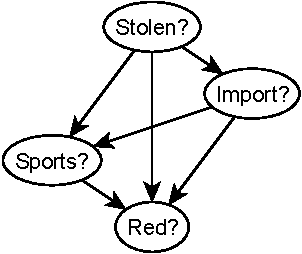
\includegraphics[scale=.75]{stolen-bayes-net}
\end{center}
\end{column}
\pause
\begin{column}{2in}
\begin{block}{Naive Bayes Network}
Assumes features are conditionally independent given the class variable
\end{block}
\begin{center}
\includegraphics[scale=.75]{stolen-naive-bayes}
\end{center}
\end{column}
\end{columns}
\end{frame}

\begin{frame}{Naive Bayes Models}
\begin{block}{Given class $C$ and features $F_1,\ldots,F_n$}
$
\begin{array}{llll}
\lefteqn{\mathbf{P}(C|F_1,F_2,\ldots,F_n)} \\
& = & \pause\alpha\mathbf{P}(F_1,F_2,\ldots,F_n|C)\mathbf{P}(C) & \mbox{Bayes' Rule} \\
& = & \pause\alpha\mathbf{P}(F_1|C)\mathbf{P}(F_2|C)\ldots\mathbf{P}(F_n|C)\mathbf{P}(C) & \mbox{Naive Bayes}
\end{array}
$
\end{block}
\pause
\vspace{-1pt}
\begin{block}{Naive Bayes models}
$\mathbf{P}(C|F_1,F_2,\ldots,F_n) = \alpha\mathbf{P}(C)\prod\limits_{i=1}^{n}\mathbf{P}(F_{i}|C)$
\end{block}
\pause
\vspace{-1pt}
\begin{block}{Training models}
\begin{itemize}
\item Find the probability of each class
\item Find the probability of each feature given the class
\end{itemize}
\end{block}
\end{frame}

\subsection{Examples}

\begin{frame}{Naive Bayes Classification}
\centering
\begin{tabular}[t]{lll|l}
Origin?  & Color? & Type?  & Stolen? \\
\hline
import   & red    & sports & yes \\
import   & red    & sports & yes \\
domestic & white  & sports & yes \\
domestic & red    & van    & yes \\
import   & red    & van    & no \\
domestic & white  & sports & no \\
\end{tabular}

\pause
\begin{block}{A domestic red sports car}
\small
$
\begin{array}{@{}l@{\hspace{.1em}}l@{\hspace{.1em}}l@{\hspace{.1em}}l@{\hspace{.1em}}l@{\hspace{.1em}}l@{\hspace{.1em}}l@{}}
\pause
P(y|d,r,s) & = & \pause\alpha P(y)P(d|y)P(r|y)P(s|y) 
           & = & \pause\alpha\cdot\pause\frac{2}{3}\cdot\pause\frac{1}{2}\cdot\pause\frac{3}{4}\cdot\pause\frac{3}{4}
           & = & \pause\frac{3}{16}\alpha
\\
\pause
P(n|d,r,s) & = & \pause\alpha P(n)P(d|n)P(r|n)P(s|n)
           & = & \pause\alpha\cdot\frac{1}{3}\cdot\frac{1}{2}\cdot\frac{1}{2}\cdot\frac{1}{2}
           & = & \pause\frac{1}{24}\alpha
\end{array}
$
\normalsize
\medskip

\pause
Predict stolen?
\pause
\alert{yes}
\hfill
\pause
At what probability?
\pause
$\alert{\frac{9}{11}} = \frac{\frac{3}{16}}{\frac{3}{16} + \frac{1}{24}}$
\end{block}
\end{frame}

\begin{frame}{Naive Bayes Exercise}
\begin{center}
\begin{tabular}[t]{cc|c}
Ends with -ed  & Initial Capital  & Part of Speech \\
\hline
no             & no               & noun \\
no             & yes              & noun \\
no             & yes              & noun \\
yes            & no               & noun \\
yes            & yes              & noun \\
no             & no               & verb \\
yes            & no               & verb \\
yes            & yes              & verb \\
\end{tabular}

\bigskip
Assign part of speech tags:
\tab\tab
\begin{tabular}[t]{cc}
John            & tripped \\
\pause
noun            & verb    \\
.84375          & .625 \\
\end{tabular}
\end{center}
\end{frame}

\subsection{Properties}

\begin{frame}{Naive Bayes Properties}
\begin{block}{Naive Bayes assumption is hardly ever true}
\begin{itemize}
\item Probability estimates of Naive Bayes are poor
\item Classification decisions are often surprisingly good
\end{itemize}
\end{block}
\pause
\begin{block}{Empirical Observations}
\begin{itemize}
\item Works best when many equally important features
\item Somewhat robust to noise (uninformative) features
\item Training and classification are typically fast
\end{itemize}
\end{block}
\end{frame}

\part{Key Ideas}
\begin{frame}{Key Ideas}
\begin{block}{Naive Bayes}
Assume features conditionally independent given class
\end{block}
\end{frame}

\end{document}


